
\frame{
\frametitle{Suodattimet}
\begin{block}{Suodatin} % Määritelmä Silvonen sivu 405
= elektroninen piiri, jonka tehtävänä on vaikuttaa läpi menevän signaalin amplitudiin ja/tai vaiheeseen eri taajuuksilla eri tavoin.
\end{block}}

\frame{
\frametitle{Toteutustapoja}
\begin{itemize}
\item Suodatin voidaan toteuttaa joko analogisesti tai digitaalisesti
\item Analoginen suodatin on aktiivinen, jos toteutuksessa on käytetty vahvistimia. Pelkistä passiivikomponenteista (käytännössä vastus, kondensaattori ja kela) koottu suodatin on passiivinen suodatin.
\end{itemize}
}

\frame{
\frametitle{Suodatintyypit}
Tavallisimmat suodatintyypit ovat
\begin{itemize}
\item Alipäästösuodatin: vaimentaa korkeita taajuuksia, päästää läpi matalat taajuudet.
\item Ylipäästösuodatin: vaimentaa matalia taajuuksia, päästää läpi korkeat taajuudet.
\item Kaistanestosuodatin: päästää läpi korkeat ja matalat taajuudet, mutta vaimentaa tietyllä välillä olevia taajuuksia.
\item Kaistanpäästösuodatin: vaimentaa liian matalia ja liian korkeita taajuuksia, mutta päästää läpi tietyllä välillä olevat taajuudet.
\item Kokopäästösuodatin: vaimennus ei ole taajuusriippuvainen, ainoastaan vaihesiirto.
\end{itemize}
}

\frame{
\frametitle{Asteluku}
\begin{itemize}
\item Suodattimen asteluku = siirtofunktion $s$:n korkein potenssi.
\item Suodattimen asteluku analogisessa suodattimessa on yleensä sama kuin suodattimen kelojen ja kondensaattorien määrä.
\item Korkeampi asteluku merkitsee yleensä jyrkempää luiskaa päästökaistan ja estokaistan välillä.
\item Päästökaistan ja estokaistan välistä pistettä kutsutaan rajataajuudeksi (engl. cut-off frequency).
\end{itemize}
}


\frame{
\frametitle{1. asteen alipäästösuodatin}
\begin{itemize}
\item Yleinen muoto $F(s)=\frac{1}{s+1}$, tällöin ominaiskulmataajuus $\omega_0=1$.
\item Sijoittamalla $s\to \frac{s}{\omega_0}$ saadaan $F(s)=\frac{1}{\frac{s}{\omega_0}+1}$
\item Voidaan toteuttaa yksinkertaisella RC-piirillä, $F(s)=\frac{\Uout}{\Uin}=\frac{1}{RCs+1}$
\item Vertaamalla siirtofunktiota ja yleistä muotoa keskenään saadaan $\omega_0=\frac{1}{RC}$
\item Ominaistaajuudella $|F(s)|=\frac{1}{\sqrt{2}}$ ja vaihekulma $-45^\circ$
\end{itemize}

\begin{picture}(50,50)(-120,0)

\hz{0,50}{R}
\vc{50,0}{C}
\du{0,0}{\Uin}
\du{65,0}{\Uout}
\hln{0,0}{50}

\end{picture}



}

\frame{
\frametitle{2. asteen alipäästösuodatin}
\begin{itemize}
\item Yleinen muoto $\frac{1}{s^2+2Ds+1} \to \frac{1}{(\frac{s}{\omega_0})^2+2D\frac{s}{\omega_0}+1}$
\item Vaimennusvakio $D$ määrää vasteen muodon, $\omega_0$ paikan (kulma)taajuusakselilla
\item Voidaan toteuttaa esim. Sallen-Key -piirillä
\item {\bf Tärkeää!} Ominaiskulmataajuudella ei välttämättä $|F(s)|=\frac{1}{\sqrt{2}}$
\end{itemize}

}

\frame{
\frametitle{Butterworth-alipäästösuodattimen asteluvun vaikutus}
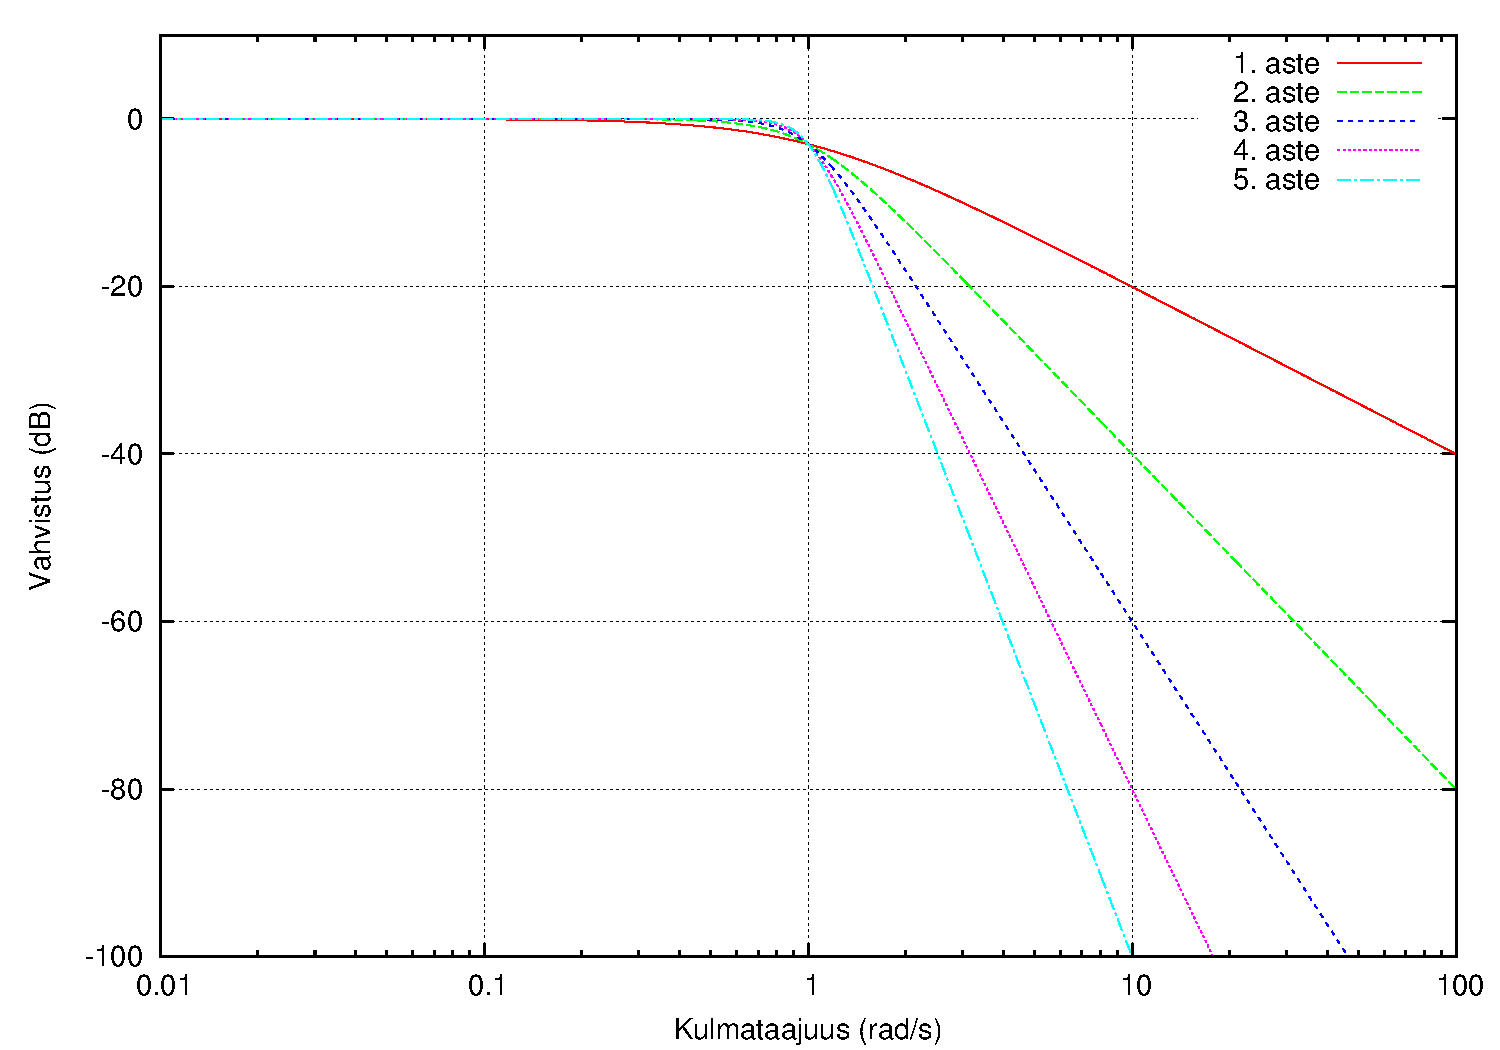
\includegraphics[height=8cm]{suodattimet_pics/bw.pdf}
}

\frame{
\frametitle{D-arvon vaikutus amplitudivasteeseen}
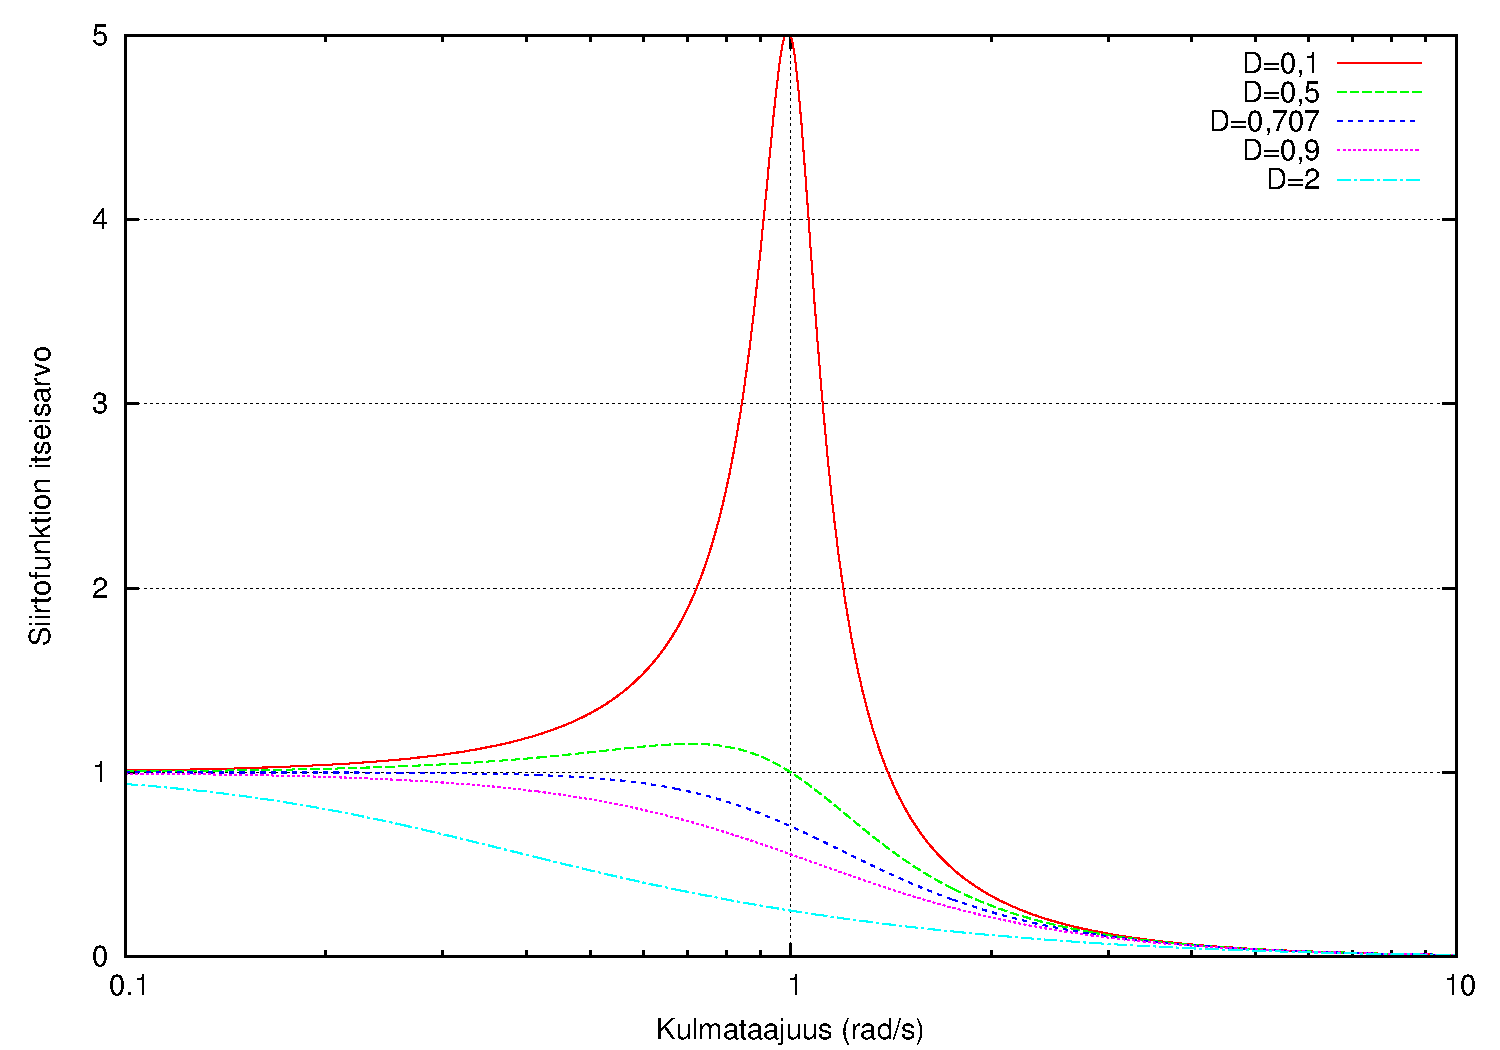
\includegraphics[height=8cm]{suodattimet_pics/d_arvo.pdf}
}

\frame{
\frametitle{Sallen-Key -alipäästösuodatin} \label{sallenkey}
\begin{center}

\begin{picture}(170,120)(0,0)

\du{0,0}{\Uin}
\hz{0,50}{R_2}
\hz{50,50}{R_1}
\vc{100,0}{C_1}
\hc{50,70}{}
\txt{75,90}{C_2}
\vo{100,50}{}{15}
\hg{100,0}
\hg{0,0}

\vln{50,50}{20}
\hln{100,100}{50}

\vln{100,70}{30}
\vln{150,60}{40}

\hln{150,60}{10}
\du{160,10}{\Uout}
\hg{160,10}

\end{picture}
\end{center}
\[
F(\jj\omega)=\frac{\Uout}{\Uin}=\frac{1}{(\jj\omega)^2C_1C_2R_1R_2+\jj\omega C_1(R_1+R_2)+1}
\]
}


\frame{
\frametitle{1. asteen ylipäästösuodatin}

\begin{itemize}
\item Siirtofunktio $\frac{s}{s+1} \to \frac{\frac{s}{\omega_0}}{\frac{s}{\omega_0}+1}$
\item Voidaan toteuttaa RC-piirillä
\end{itemize}

\begin{picture}(50,50)(-120,0)

\hc{0,50}{C}
\vz{50,0}{R}
\du{0,0}{\Uin}
\du{65,0}{\Uout}
\hln{0,0}{50}

\end{picture}

}

\frame{
\frametitle{2. asteen ylipäästösuodatin}
\begin{itemize}
\item Yleinen muoto $\frac{s^2}{s^2+2Ds+1} \to \frac{(\frac{s}{\omega_0})^2}{(\frac{s}{\omega_0})^2+2D\frac{s}{\omega_0}+1}$
\item Voidaan toteuttaa esim. Sallen-Key -piirillä
\item {\bf Tärkeää!} Ominaiskulmataajuudella ei välttämättä $|F(s)|=\frac{1}{\sqrt{2}}$
\end{itemize}
}


\frame{
\frametitle{Mitoitus ja taajuusmuunnokset}
\begin{itemize}
\item Haluttu piste ominaiskäyrällä voidaan siirtää muualle sijoittamalla $s\to s\frac{f_{\rm vanha}}{f_{\rm uusi}}$
\item Esimerkiksi jos siirtofunktion puolen tehon piste sijaitsee paikassa $\omega=42$ ja se halutaan taajuudelle
$f=500\Hz$, sijoitetaan siirtofunktioon jokaisen $s$:n paikalle $s\frac{42}{2\pi\cdot 500}$
\item Osoittajan kertominen vakiokertoimella ei vaikuta amplitudivasteen muotoon eikä vaiheeseen.
\item Mitoittamisen lähtökohtana on nimittäjäpolynomi, joka katsotaan taulukkokirjasta. Esim:
\begin{itemize}
\item Butterworth
\item Bessel
\item Legendre
\item \ldots
\end{itemize}
\end{itemize}
}




\frame{
\frametitle{Näin mitoitan suodattimen}
Esimerkki: Suunnittele toisen asteen Butterworth-alipäästösuodatin, jonka puolen tehon piste
on taajuudella 500 Hz. Toisen asteen Butterworth-polynomi on $(s^2+\sqrt{2}s+1)$.\\

Ratkaisun kulku:
\begin{enumerate}
\item Selvitetään, millä taajuudella sijaitsee puolen tehon piste alkuperäisellä siirtofunktiolla
\item Siirretään piste taajuudelle 500 Hz
\item Ratkaistaan $D$ ja $\omega_0$
\item (Rakennetaan piiri)
\end{enumerate}
}

\frame{
\frametitle{Selvitetään puolen tehon piste ja siirretään se}
Tasajännitteellä ($\omega=0$) vahvistus on 1, joten puolen tehon kulmataajuus on
\[
\Bigg|\frac{1}{s^2+\sqrt{2}s+1}\Bigg|=\frac{1}{\sqrt{2}}, s=\jj\omega_{1/2},
\]
josta ratkeaa $\omega_{1/2}=1$. Tämä piste saadaan siirrettyä taajuudelle 500 Hz tekemällä sijoitus
\[
s\to s\frac{1}{2\pi\cdot 500},
\]
jolloin siirtofunktioksi saadaan
\[
\frac{1}{(\frac{s}{2\pi\cdot 500})^2+\sqrt{2}\frac{s}{2\pi\cdot 500}+1}.
\]
}

\frame{
\frametitle{Ratkaistaan $\omega_0$ ja $D$}
Vertaamalla saatua siirtofunktiota yleiseen muotoon
\[
\frac{1}{(\frac{s}{2\pi\cdot 500})^2+\sqrt{2}\frac{s}{2\pi\cdot 500}+1}=\frac{1}{(\frac{s}{\omega_0})^2+2D\frac{s}{\omega_0}+1}
\]
nähdään, että $\omega_0=2\pi\cdot 500\approx 3140$ ja $D=\frac{1}{\sqrt{2}}$.
}

 \frame{
 \frametitle{Esimerkki}
\begin{center}
\begin{picture}(170,110)(0,0)

\du{0,0}{\Uin}
\hc{0,50}{C_2}
\hc{50,50}{C_1}
\vz{100,0}{R_1\hspace{-1mm}}
\hz{50,70}{}
\txt{75,90}{R_2}
\vo{100,50}{}{15}
\hg{100,0}
\hg{0,0}

\vln{50,50}{20}
\hln{100,100}{50}

\vln{100,70}{30}
\vln{150,60}{40}

\hln{150,60}{10}
\du{160,10}{\Uout}
\hg{160,10}

\end{picture}

\end{center}

Osoita, että kuvan piirin siirtofunktio on 2. asteen ylipäästöfunktio eli muotoa
\[
F(s)=\frac{\Uout}{\Uin}=\frac{(\frac{s}{\omega_0})^2}{(\frac{s}{\omega_0})^2+2D\frac{s}{\omega_0}+1}
\]
ja laske arvot $D$ ja $\omega_0$ (komponenttiarvojen funktiona). 


\tiny $\omega_0=\frac{1}{\sqrt{C_1C_2R_1R_2}}$ ja $D=\frac{1}{2}\frac{R_2(C_1+C_2)}{\sqrt{C_1C_2R_1R_2}}$}